\documentclass[11pt,a4paper]{article}

\usepackage{graphicx}
\usepackage{amsmath}
\usepackage{hyperref}
\usepackage{enumitem}
\usepackage{geometry}
\usepackage{fancyhdr}
\usepackage{sectsty}
\usepackage[T1]{fontenc}
\usepackage{titlesec}
\usepackage{float}

\sectionfont{\centering\MakeUppercase}

\geometry{top=2.54cm, bottom=2.54cm, left=1.91cm, right=1.91cm}

\title{Comparison of a Smaller Specialized Segmentation Model (U-Net) to an Advanced Fine-Tuned Model (TransUNet)}
\author{
    Vinay Kumar\\
    MAI Programme\\
    University of Amberg-Weiden\\
    Amberg
}

\begin{document}

\maketitle

\vspace{0.4cm}
\section{abstract}
\raggedright
The project involves segmenting MRI images using U-Net and TransUNet models. These models are essential in deep learning for identifying regions of interest in MRI scans, crucial for any medical application. The dataset consists of preprocessed MRI images with their masks, which were quality-checked and balanced. The experiments demonstrated that biomedical image segmentation tasks could be implemented using models like U-Net and TransUNet, where additional dependencies create compact layers through convolution and up-sampling. Data preprocessing, addressing issues like missing data and sample balancing, played a significant role, especially in image resizing. After training and validating the models, unbiased validation of the developed PyTorch models ensured accurate and robust MRI image segmentation. The primary challenges included handling missing data, unbalanced datasets, and resizing images. This project's success in medical image segmentation using U-Net and TransUNet paves the way for further investigation into various designs for broader applications in medical imaging.

\vspace{0.6cm}
\section{Introduction}
\raggedright
Medical image segmentation is one of the most significant tasks in medical imaging, enabling precise identification and location of regions or structures of interest. Accurate segmentation of MRI images is crucial for several clinical applications in disease diagnosis, treatment planning, and observation. This project implements deep learning techniques on U-Net and TransUNet architectures for high-accuracy MRI image segmentation. The focus on these models aims to improve the segmentation procedure by yielding more well-defined and reliable results.

\vspace{0.4cm}
\textbf{Note:} All these tasks were performed on OTH KI-Server.
\vspace{5.0cm}

\section{Project Planning}
\raggedright
The project is divided into several phases to ensure structured progress and timely completion. Each phase is described below:

\begin{itemize}
    \item Project Initiation and Setup
    \item Data Collection and Preprocessing
    \item Model Development
    \item Model Training and Evaluation
    \item Results Analysis and Visualization
    \item Conclusion and Future Aspects
\end{itemize}

\subsection{Project Initiation and Setup}
The initial phase of the project involved defining the objectives, scope, and deliverables. This included a comprehensive literature review to understand the current state of medical image segmentation and the selection of suitable deep learning models. The virtual environment was set up for this task, but due to the large dataset, all tasks were performed on OTH KI-Server, which already had the necessary software libraries and tools such as PyTorch installed.

\subsection{Data Collection and Preprocessing}
\subsubsection{Source of Data}
The MRI images and corresponding masks used in this project were downloaded from Kaggle. The dataset is available at this \href{https://www.kaggle.com/}{Kaggle link} [1].

The dataset contains brain MRI images along with manual FLAIR abnormality segmentation masks. The images were obtained from The Cancer Imaging Archive (TCIA) and correspond to 110 patients included in The Cancer Genome Atlas (TCGA) lower-grade glioma collection with at least fluid-attenuated inversion recovery (FLAIR) sequence and genomic cluster data available. Tumor genomic clusters and patient data are provided in the 'data.csv' file.

\subsubsection{Data Preprocessing}
\begin{itemize}
    \item Images and masks were read using OpenCV, a library for handling computer vision tasks. The code for data loading and preprocessing was utilized from this \href{https://www.kaggle.com/code/arham23/brain-mri-segmentation-eda-and-unet-unet-results/notebook}{Kaggle Code} [2].
    \item Some images were discovered that lacked corresponding masks, and similarly, there were masks without matching images. We used counters and lists to track these discrepancies, removing these incomplete data points from both the training and evaluation processes.
    \item The dataset was balanced by maintaining an equal number of positive samples (images with masks) and negative samples (images without masks). Achieving this balance is essential for training a robust segmentation model.
    \item A significant challenge was resizing the images while maintaining the integrity of the regions of interest. Images and masks were resized to a consistent dimension suitable for input into the U-Net and TransUNet models.
    \item Some images were discovered that lacked corresponding masks, and similarly, there were masks without matching images. Data augmentation techniques were applied to artificially increase the size of the training dataset and improve model generalization. 
\end{itemize}

\begin{figure}[H]
    \centering
    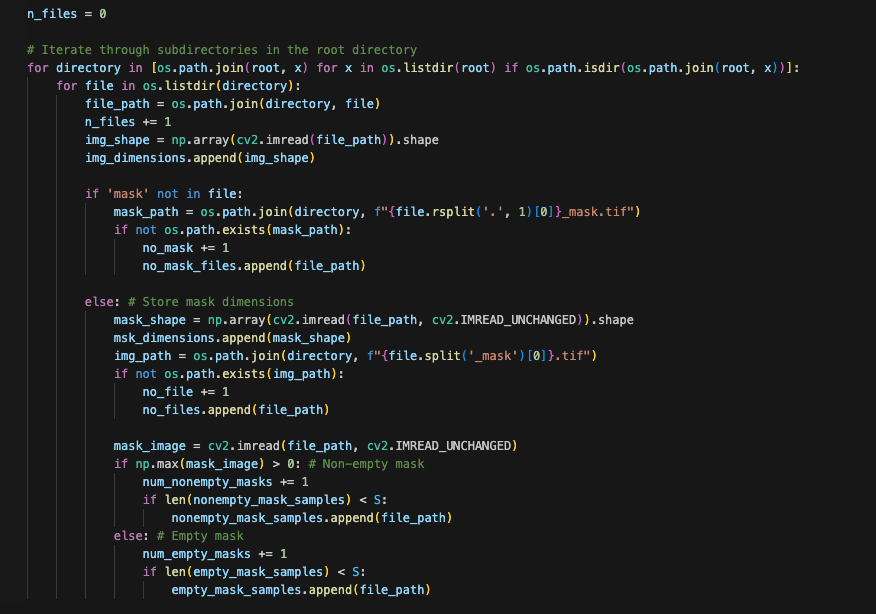
\includegraphics[width=\linewidth]{data_def.png}
    \caption{Data defining}
    
\end{figure}
\vspace{1.0cm}
\begin{itemize}
    \item The MRI images show cross-sectional views of the brain, while the masks highlight specific regions of interest, such as tumor areas
    \item MRI images are in color, providing detailed anatomical information with various intensity levels to highlight different tissue types
    \item The images and masks are resized to a consistent dimension, in this case, 224x224 pixels.
    \item Some MRI images have corresponding masks with segmented regions (highlighted in yellow in the provided image). These regions represent abnormalities or areas of interest, such as tumors
    \item The dataset includes a variety of brain scans, showing different slices and anatomical structures
    
\end{itemize}

\begin{figure}[H]
    \centering
    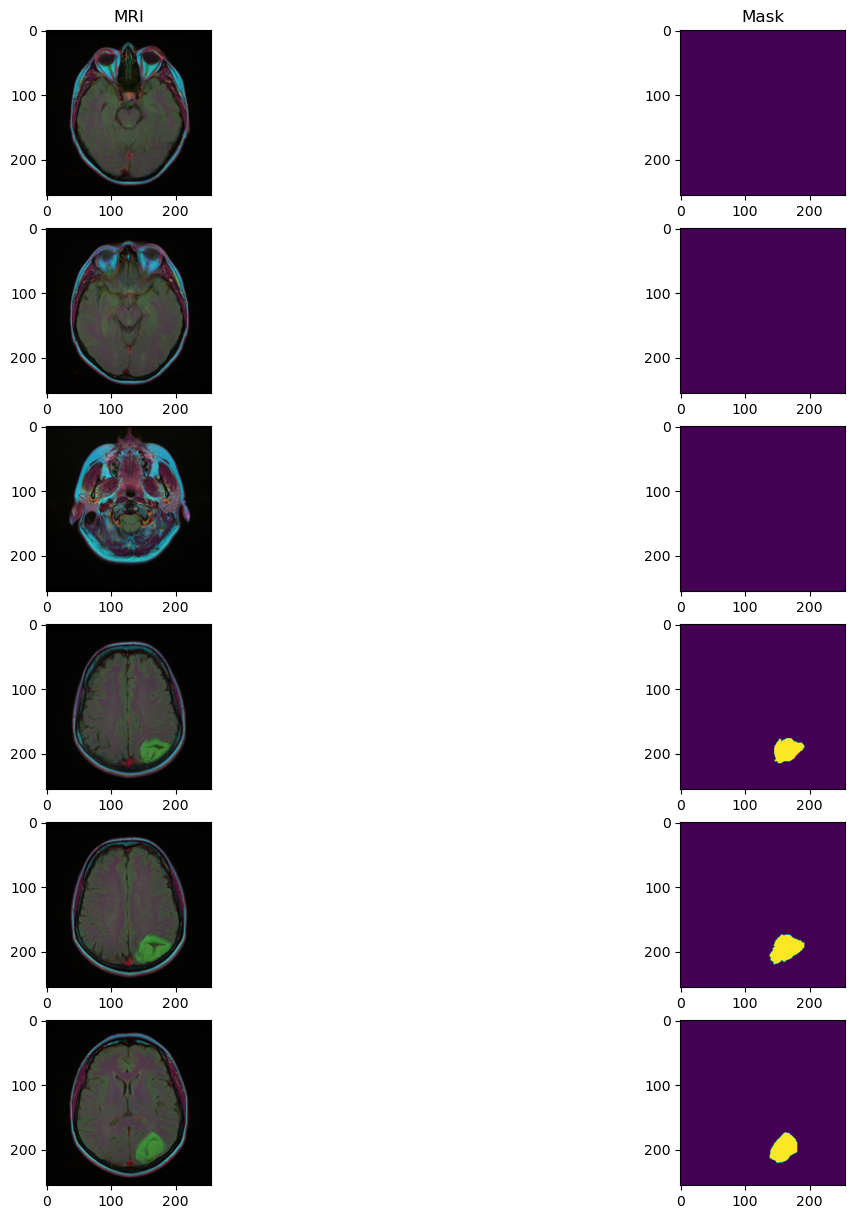
\includegraphics[width= 0.9\linewidth]{output.png}
    \caption{MRI Images}
    
\end{figure}

\vspace{1.0cm}
\subsection{Data Loaders}
Data loaders are essential for efficiently managing and feeding data into models during training and evaluation
\begin{itemize}
    \item Training deep learning models on entire datasets at once is computationally impractical due to memory constraints
    \item To ensure that the model does not learn any unintended sequence or pattern in the data, data loaders can shuffle the dataset before each epoch
    \item Data loaders automatically create batches of data from the dataset, removing the need for manual batch creation and ensuring consistent batch sizes
    \item By leveraging multiple workers, data loaders can load and preprocess data in parallel, significantly speeding up the data pipeline and ensuring the GPU is efficiently utilized without waiting for data
    \item Data loaders can apply transformations and augmentations to the data in real-time during training
    \item There is a consistent and uniform way of handling data across different phases of the training pipeline (training and validation), ensuring that the model receives data in a standardized format
\end{itemize}
\vspace{0.5cm}


\subsection{Model Defining}
\subsubsection{Overview of U-Net}
U-Net is a convolutional neural network architecture designed for image segmentation tasks. It consists of two main parts: the contracting path (encoder) and the expanding path (decoder).
\linebreak
This architecture is particularly effective for biomedical image segmentation due to its ability to capture both local and global features. The code is available at this where I have copied the architecture \href{https://github.com/uygarkurt/UNet-PyTorch/blob/main/unet.py}{Github link} [3]
\vspace{0.4cm}
\begin{itemize}
    \item \textbf{DoubleConv:} This block performs two consecutive convolution operations, which help in learning more complex features. ReLU activations introduce non-linearity, allowing the model to capture non-linear patterns.
    \item \textbf{DownSample:} Combines double convolutions with max-pooling. Max-pooling reduces the spatial dimensions of the feature maps, helping the network to capture hierarchical features and reducing computational complexity.
    \item \textbf{UpSample:} Upsamples the feature maps using transposed convolution, then applies double convolutions. The upsampled feature map is concatenated with the corresponding feature map from the encoder, which helps in retaining spatial information.
    \item \textbf{UNet Class:}
    \begin{itemize}
        \item \textbf{Encoder Path:} The encoder path consists of sequential downsampling blocks, which progressively reduce the spatial dimensions while increasing the depth of the feature maps.
        \item \textbf{Bottleneck:} Acts as a bridge between the encoder and decoder, processing the most compressed form of the feature maps.
        \item \textbf{Decoder Path:} The decoder path consists of upsampling blocks, which progressively increase the spatial dimensions while decreasing the depth of the feature maps
        \item \textbf{Output Layer:} A final convolutional layer reduces the number of channels to the desired number of output classes, producing the segmentation map.
    \end{itemize}
\end{itemize}
\begin{figure}[H]
    \centering
    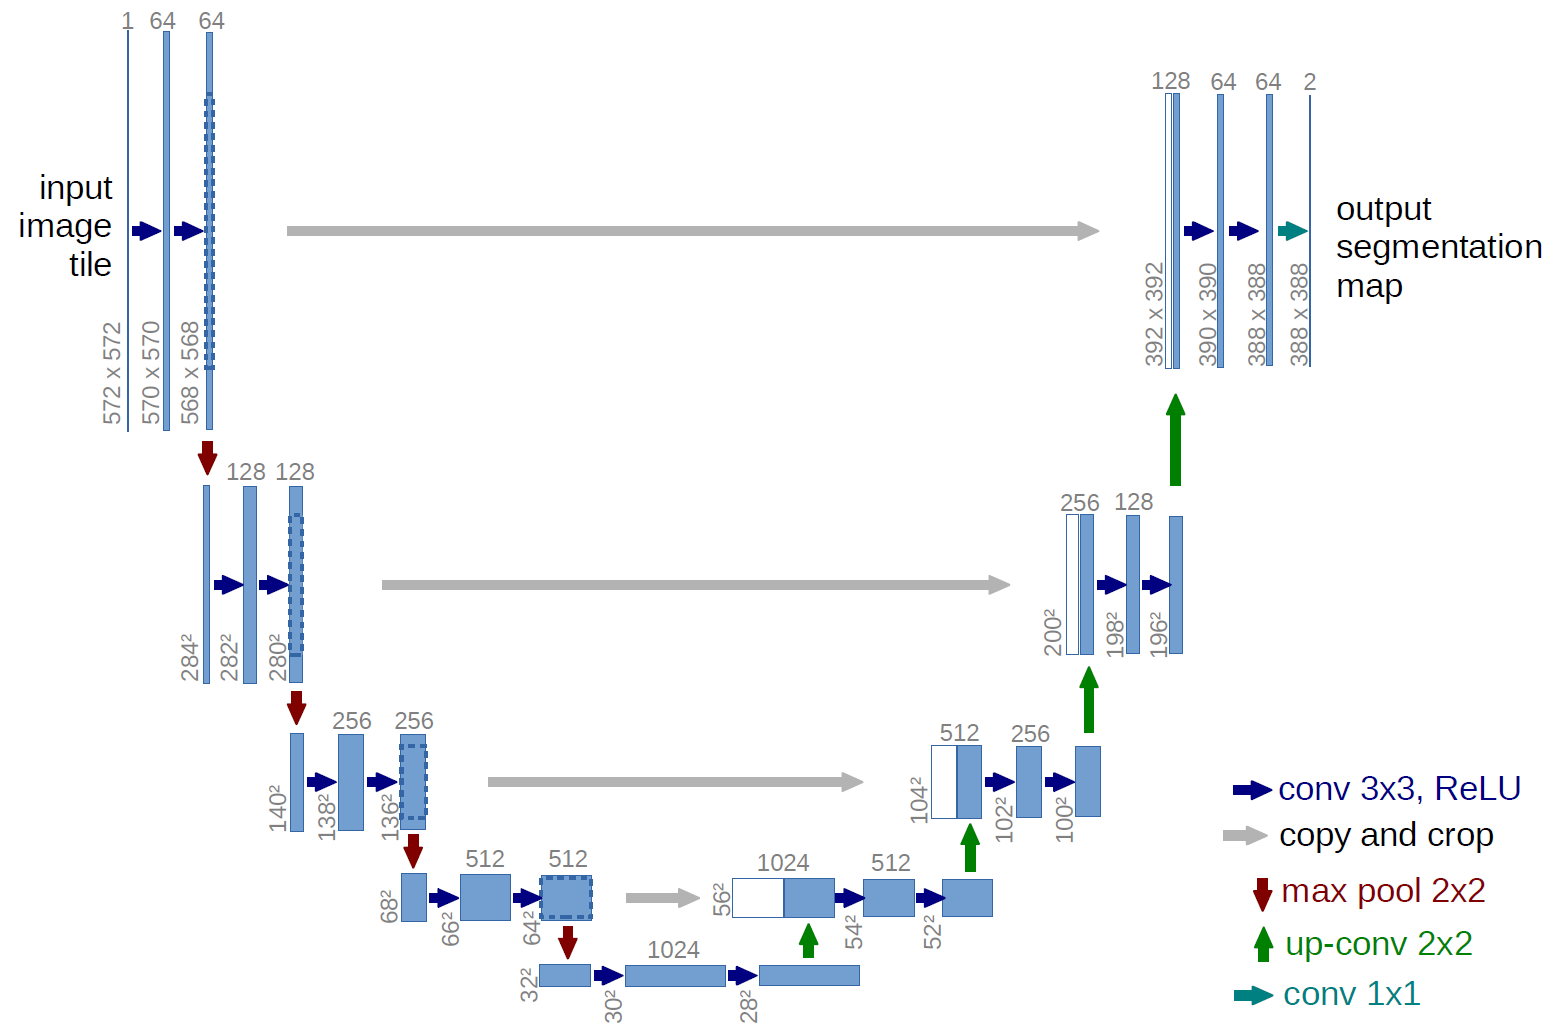
\includegraphics[width= 0.9\linewidth]{u-net-architecture.png}
    
    \caption{U-Net Architecture \newline \space Source: \href{https://lmb.informatik.uni-freiburg.de/people/ronneber/u-net/}{3}}
    
\end{figure}
\vspace{0.6cm}
U-Net architecture is symmetrical in layout, featuring skip connections, and is very suitable for image segmentation. The following code snippet initializes such an architecture in PyTorch using double convolutions, downsampling, and upsampling processes connected by skip links. The architecture enables large-scale feature capturing.
\vspace{0.2cm}
\linebreak
To detect and distinguish between various parts within a picture, the U-Net architecture makes use of this specific characteristic. Because precise segmentation of anatomical structures is essential in medical picture interpretation, this makes it very helpful. In general, U-Net is an encoding-decoding structure whose downsampling path allows for context capturing and its upsampling path allows for exact localization.
\vspace{0.2cm}
\linebreak
The skip connections result in high resolution characteristics from the contracting path, these features need to be combined with the upsampled output for more accurate segmentation. The accuracy and reliability of the final segmentation results should increase because U-Net will be trained on a range of picture segmentation tasks in this PyTorch implementation.

\begin{figure}[H]
    \centering
    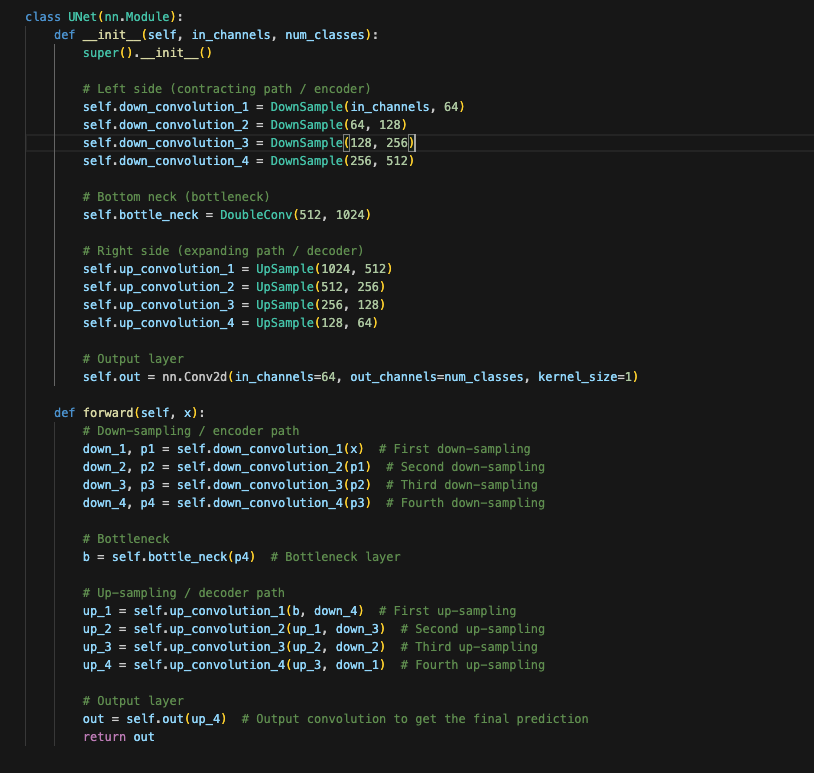
\includegraphics[width= 0.9\linewidth]{model_imple.png}
    \caption{U-Net Model}
    
\end{figure}
\vspace{0.6cm}
\subsubsection{Overview of TransUNet}
TransUNet is a hybrid architecture that leverages both Vision Transformers (ViTs) and Convolutional Neural Networks (CNNs). The ViT captures global context by processing the entire image as a sequence of patches, while the CNN decoder reconstructs the segmentation map by upsampling the feature maps obtained from the ViT
\begin{itemize}
    \item The Transformer component helps in understanding the global context of the image, which is crucial for segmenting complex structures in medical images.
    \item By combining CNNs and Transformers, TransUNet can potentially achieve higher accuracy in segmentation tasks compared to using CNNs alone
    \item The architecture can be adapted for various image segmentation tasks beyond medical imaging
\end{itemize}
\begin{figure}[H]
    \centering
    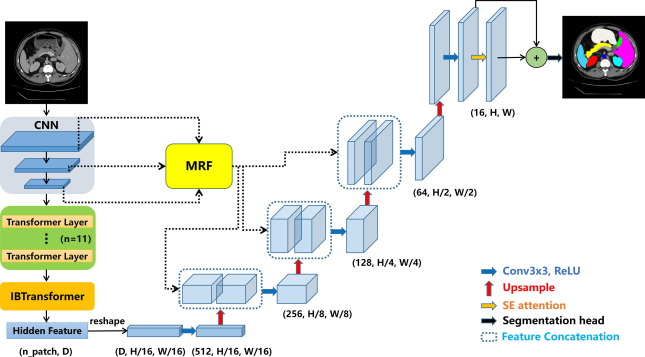
\includegraphics[width= 0.9\linewidth]{transUnet_arc.jpg}
    
    \caption{TransUNet Architecture \newline \space Source: \href{https://www.sciencedirect.com/science/article/pii/S1319157823000411}{4}}
    
\end{figure}
\vspace{0.4cm}
\begin{itemize}
    \item Combines the local feature extraction capabilities of CNNs with the global context understanding of Transformers.
    \item Utilizes a Transformer encoder to capture long-range dependencies in the input image.
    \item Uses a convolutional decoder (similar to U-Net) to reconstruct the high-resolution segmentation map.
    \item Incorporates skip connections to retain spatial information from the encoder layers.
\end{itemize}
\begin{figure}[H]
    \centering
    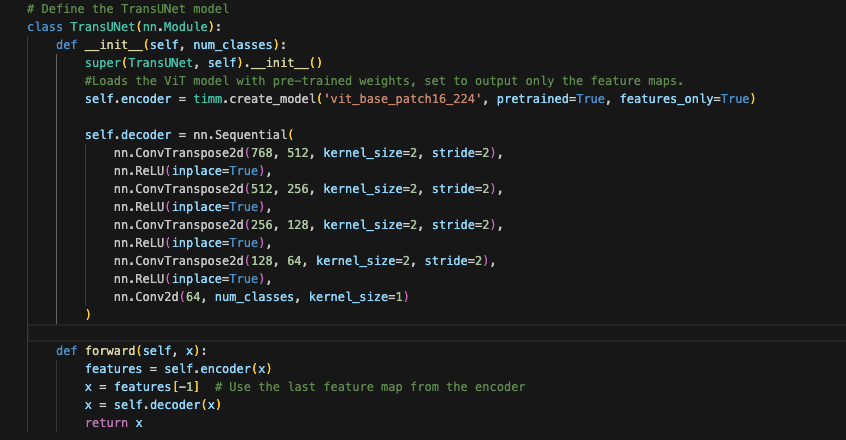
\includegraphics[width= 0.9\linewidth]{transUnet_imp.png}
    \caption{TransUNet Model}
    
\end{figure}
I implemented a fine-tuning model using TransUNet for medical image segmentation. The TransUNet model combines a pre-trained Vision Transformer (ViT) encoder with a CNN decoder. The ViT encoder, loaded with pre-trained weights, extracts global features from the input images, while the CNN decoder upsamples these features to reconstruct high-resolution segmentation maps
\vspace{0.2cm}
\linebreak
Fine-tuning allows leveraging the learned features from the pre-trained ViT, enhancing the model's performance on the specific segmentation task. This hybrid approach captures both global context and local details, making it effective for accurate and detailed medical image segmentation.
\vspace{0.6cm}
\subsection{Model Training and Evaluation}
\begin{itemize}
    \item The model training process involves training and evaluating two models, TransUNet and UNet, over multiple epochs to achieve optimal segmentation performance
    \item I have used separate AdamW optimizers for each model.
    \item Learning rates are set to \(5 \times 10^{-5}\) for TransUNet and \(3 \times 10^{-4}\) for UNet.
    \item The training loop iterates over a specified number of epochs (40 in this case). In each epoch, the models are trained on the training dataset and evaluated on the validation dataset
    \item During training, the models are set to training mode, and the optimizer gradients are reset before each batch (8 in this case).
    \item The forward pass computes model outputs, where the loss is calculated and afterward backpropagated for updating model parameters. It involves sending the input data through the network to receive predictions; these are compared with actual values to compute the loss
    \item The calculated loss will then be used to adjust the weights of the model in a process called backpropagation to improve the model's performance over time by minimizing the loss.

\end{itemize}
\begin{figure}[H]
    \centering
    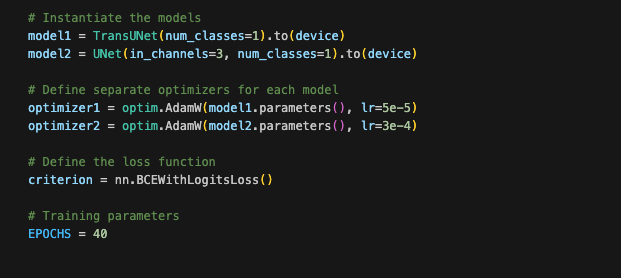
\includegraphics[width= 0.9\linewidth]{parameters.png}
    \caption{parameters}
    
\end{figure}
\vspace{0.5cm}
\subsubsection{Evaluation}

\begin{itemize}
    \item The evaluation process assesses the performance of the trained models, TransUNet and UNet, on the validation dataset to ensure they generalize well to unseen data
    \item The evaluation is conducted at the end of each training epoch to monitor progress and make adjustments if necessary.
    \item \textbf{Matrics Calculation}
    \begin{itemize}
        \item \textbf{Loss:} The same loss function \textbf{(BCEWithLogitsLoss)} used during training is applied to quantify the difference between predictions and actual masks.
        \item \textbf{IoU (Intersection over Union):} Measures the overlap between predicted and ground truth masks, providing insight into the model's accuracy. 1 indicates perfect overlap, and 0 indicates no overlap
        \item \textbf{Dice Coefficient:} Another overlap metric that is particularly sensitive to class imbalances, often used in medical image segmentation. It gives a better measure of accuracy when there are unequal class distributions
        \item \textbf{Precision, Recall, and F1 Score:} Precision measures the proportion of true positive predictions, recall measures the proportion of actual positives correctly identified, and F1 score provides a balance between precision and recall
        
    \end{itemize}
    \item Matrics helps us in understanding how well the model identifies the regions of interest versus the background, which is critical for applications like medical image segmentation where accuracy is paramount.

\end{itemize}
\begin{figure}[H]
    \centering
    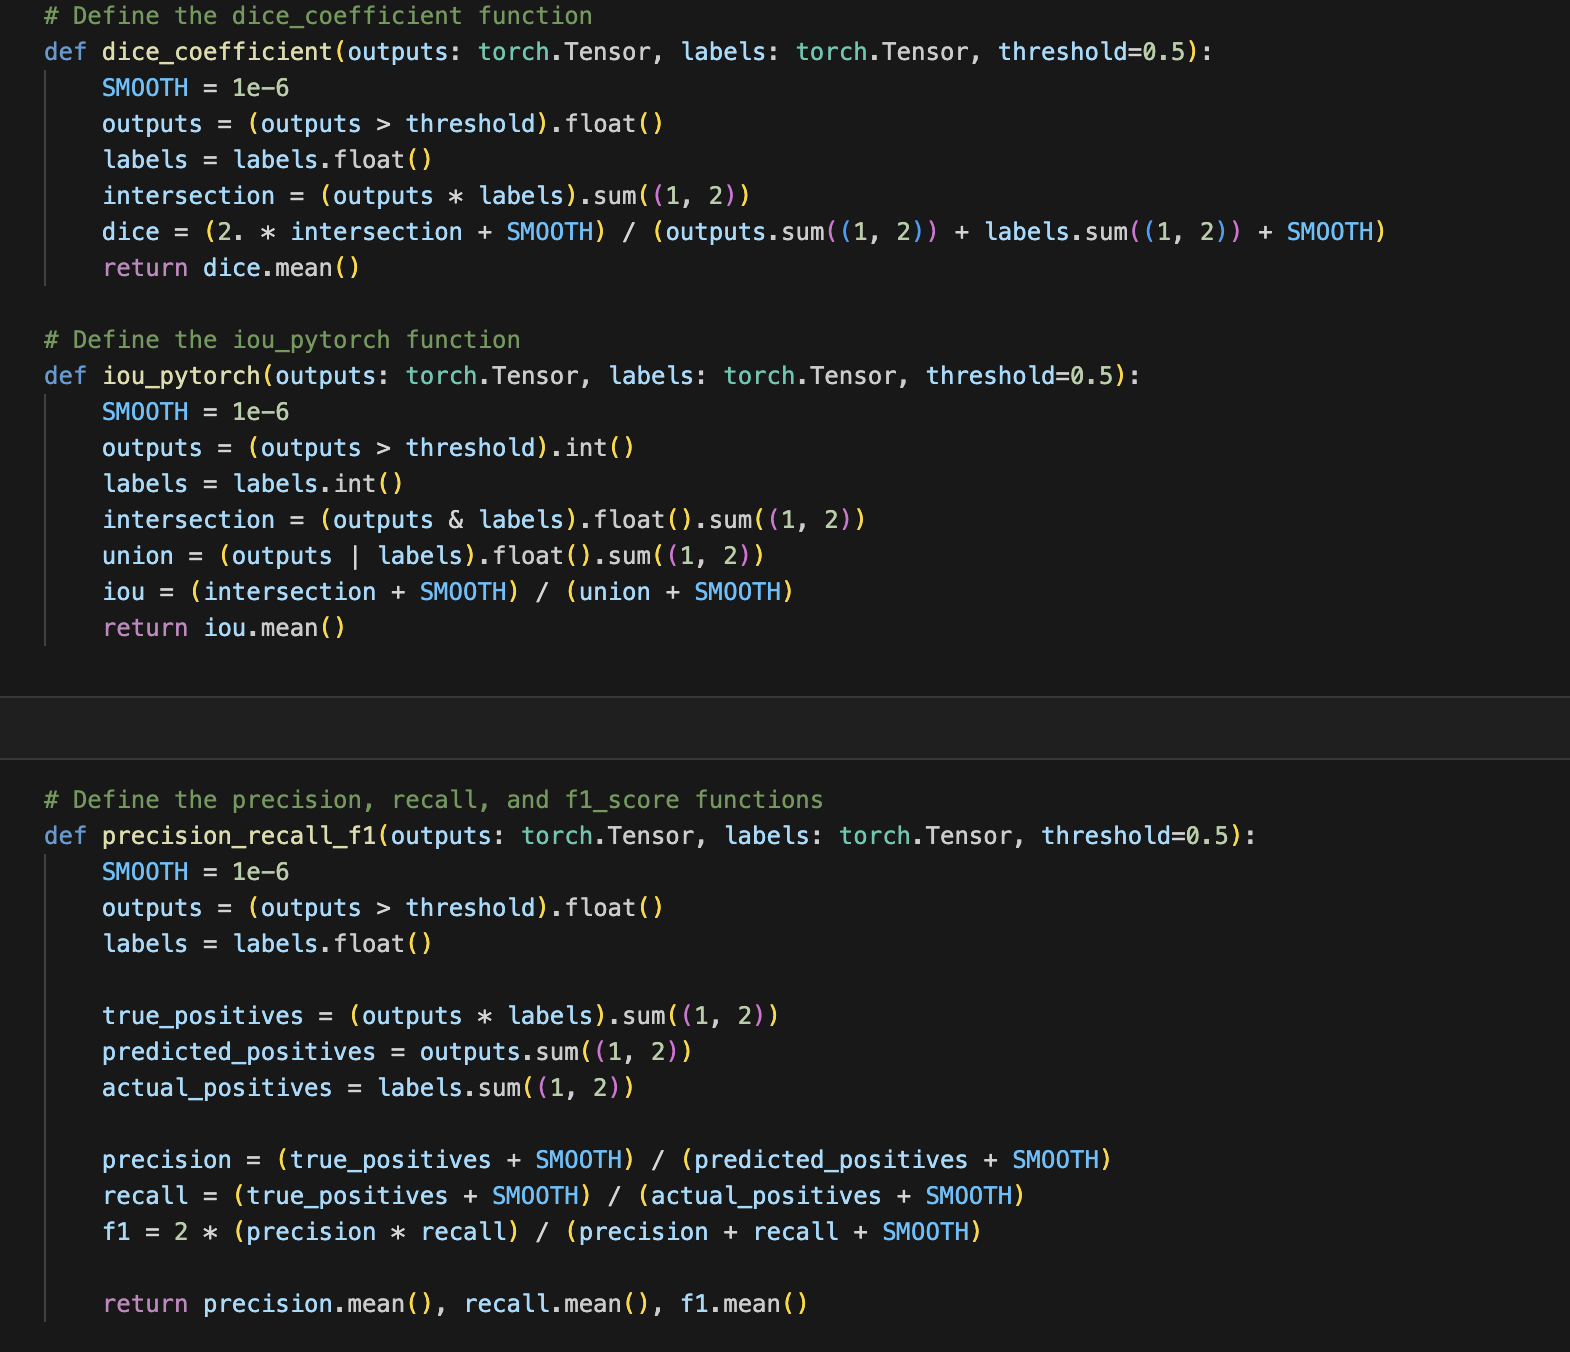
\includegraphics[width= 0.82\linewidth]{martics.png}
    
    \caption{Matrics defining \newline  \space Source: \href{https://www.kaggle.com/code/arham23/brain-mri-segmentation-eda-and-unet-unet-results/notebook}{2}}
    
\end{figure}

Confusion matrices play a key role in this process by providing detailed insights into the model's classification performance, identifying specific errors, and facilitating the calculation of important metrics like precision, recall, F1 score, IoU, and Dice coefficient
\vspace{0.2cm}
\linebreak
These metrics are vital for understanding the model's strengths and weaknesses, guiding improvements, and ensuring robust segmentation performance.
\vspace{0.9cm}
\subsection{Results Analysis and Visualization}
\subsubsection{Result Analysis}
\begin{itemize}
    \item \textbf{Train Loss}
    \begin{itemize}
        \item The training loss for both models (TransUNet and UNet) decreases significantly in the initial epochs, indicating that the models are learning to fit the training data effectively
        \item As training progresses, the loss continues to decrease but at a slower rate, eventually stabilizing towards the later epochs
        \item The overall trend shows a steady reduction in loss, which is a positive indication of effective learning 
    \end{itemize}
\end{itemize}
\begin{figure}[H]
    \centering
    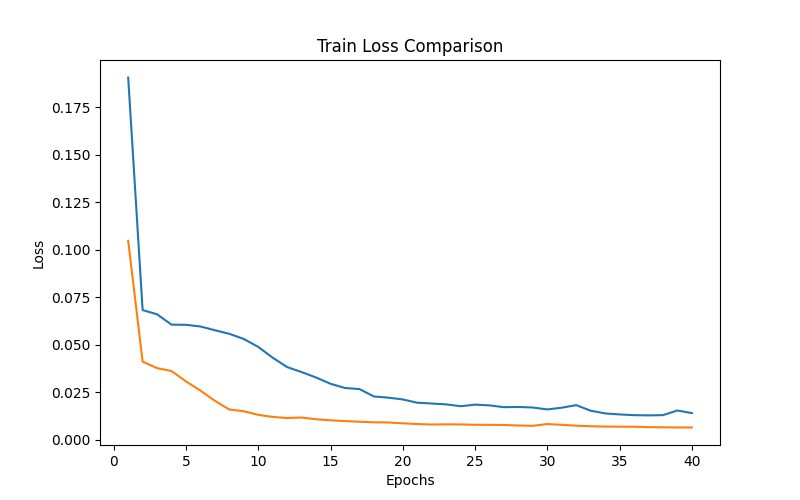
\includegraphics[width= 0.9\linewidth]{train_loss.png}
    \caption{Train Loss (Blue refers to U-Net and orange refers to TransUNet)}
    
\end{figure}
\pagebreak
\begin{itemize}
    \item \textbf{Validation Loss}
    \begin{itemize}
        \item The validation loss for both models also shows a decreasing trend over the epochs, demonstrating that the models are generalizing well to unseen data
        \item There are some fluctuations in the validation loss, particularly in the middle epochs, which could be due to the models encountering more challenging samples in the validation set
        \item The validation loss stabilizes towards the later epochs, with both models achieving relatively low loss values, indicating good generalization
    \end{itemize}
\end{itemize}
\begin{figure}[H]
    \centering
    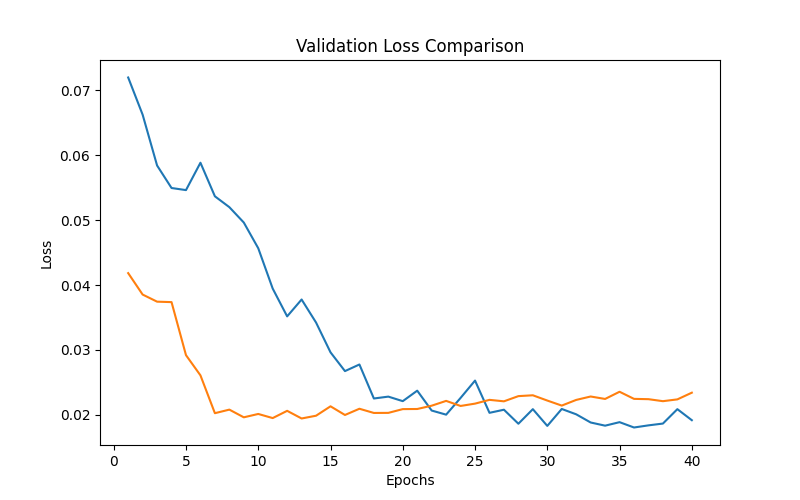
\includegraphics[width= 0.9\linewidth]{val_loss.png}
    \caption{Val Loss (Blue refers to U-Net and orange refers to TransUNet)}
    
\end{figure}
\pagebreak
\begin{itemize}
    \item \textbf{Validation IoU}
    \begin{itemize}
        \item Both models show an increasing trend in IoU over the epochs, indicating improved performance.
        \item TransUNet (represented in orange) quickly achieves high IoU, reaching above 0.92 within the first 10 epochs and stabilizing around 0.92-0.93
        \item UNet (represented in blue) shows a gradual increase in IoU, stabilizing around 0.90-0.91 towards the end of the training period
        
    \end{itemize}
\end{itemize}
\begin{figure}[H]
    \centering
    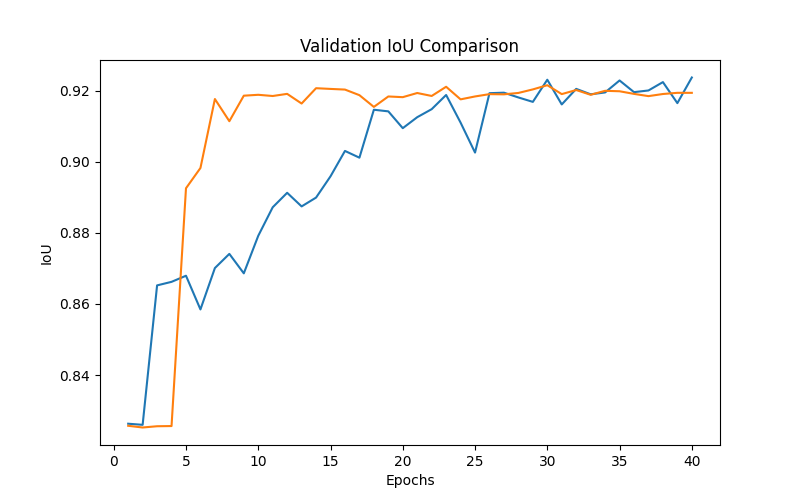
\includegraphics[width= 0.9\linewidth]{IOU.png}
    \caption{IoU Comparison (Blue refers to U-Net and orange refers to TransUNet)}
\end{figure}
\pagebreak
\begin{itemize}
    \item \textbf{Validation Precision}
    \begin{itemize}
        \item Both models show high precision throughout the training period, with values oscillating between 0.96 and 1.0
        \item TransUNet (in orange) maintains very high precision (>0.98) consistently, with minor fluctuations
        \item UNet (in blue) shows more variability in precision, with occasional drops below 0.97 but generally staying above 0.97
        \item The high precision of TransUNet indicates it makes fewer false positive errors, consistently predicting positive regions accurately
    \end{itemize}
\end{itemize}
\begin{figure}[H]
    \centering
    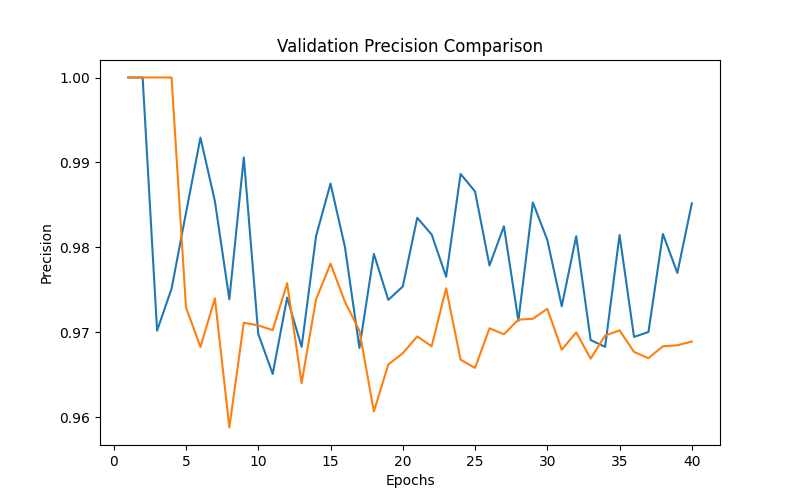
\includegraphics[width= 0.9\linewidth]{Precision.png}
    \caption{Precision Comparison (Blue refers to U-Net and orange refers to TransUNet)}
\end{figure}
\pagebreak
\begin{itemize}
    \item \textbf{Validation Recall}
    \begin{itemize}
        \item Both models show an increasing trend in recall over the epochs, indicating improved ability to identify positive regions
        \item TransUNet (in orange) achieves high recall quickly, stabilizing around 0.93-0.94
        \item UNet (in blue) shows a gradual increase in recall, reaching around 0.91 towards the end of the training period
    \end{itemize}
\end{itemize}

\begin{figure}[H]
    \centering
    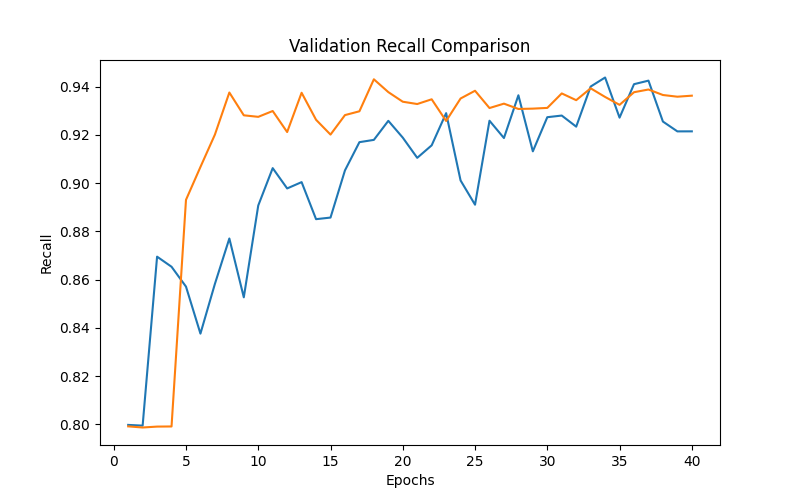
\includegraphics[width= 0.9\linewidth]{recall.png}
    \caption{Recall Comparison (Blue refers to U-Net and orange refers to TransUNet)}
\end{figure}
\vspace{0.9cm}
\begin{itemize}
    \item \textbf{Summary}
    \begin{itemize}
        \item Shows rapid improvement and high performance across all metrics
        \item Consistently achieves high IoU, precision, and recall, indicating strong segmentation capabilities with fewer errors
        \item These metrics highlight the effectiveness of TransUNet in capturing both global and local features, leading to better segmentation performance compared to UNet
        \item The high and consistent values across IoU, Precision, and Recall metrics underscore TransUNet's robustness and reliability in medical image segmentation tasks
    \end{itemize}
\end{itemize}
\vspace{8.9cm}
\subsubsection{Result Visualization}
\begin{itemize}
    \item \textbf{Result of U-Net}
\end{itemize}
\begin{figure}[H]
    \centering
    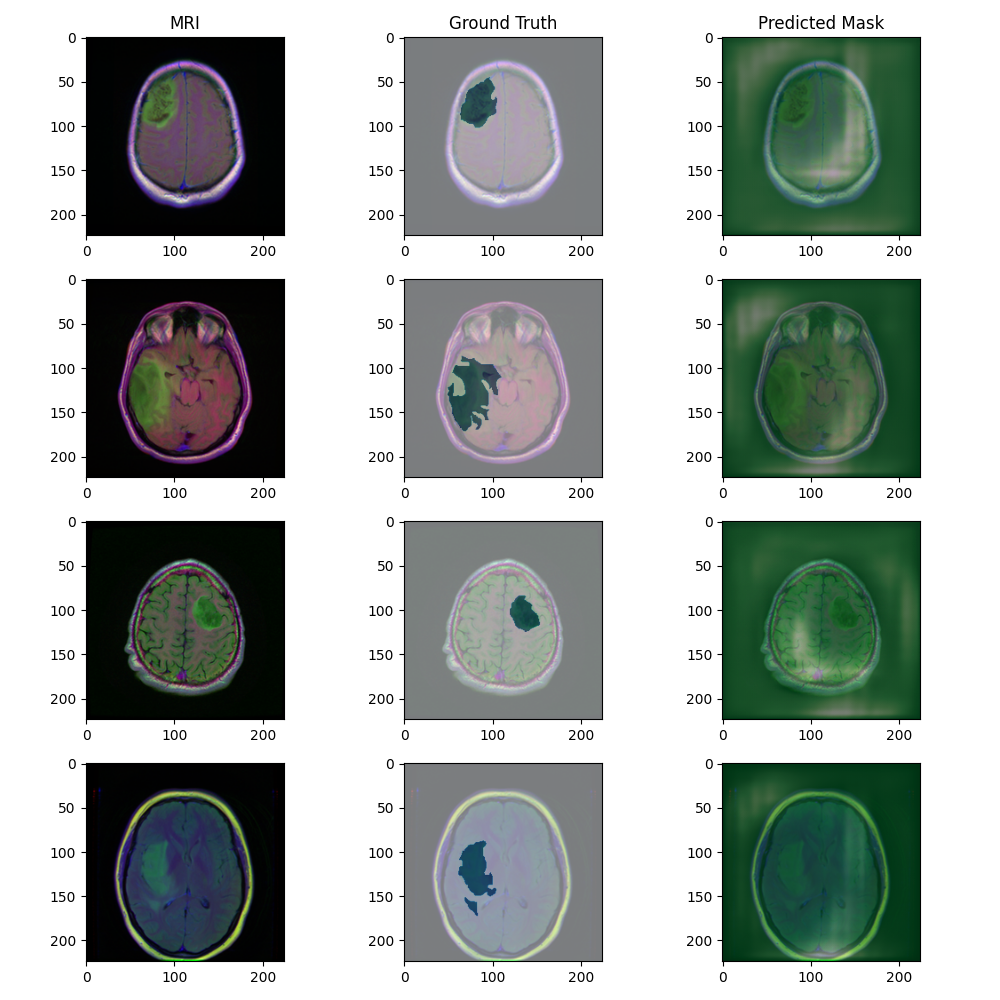
\includegraphics[width= 0.9\linewidth]{Unet.png}
    \caption{Unet Result}
\end{figure}
\pagebreak
\begin{itemize}
    \item \textbf{Result of TransUNet}
\end{itemize}
\begin{figure}[H]
    \centering
    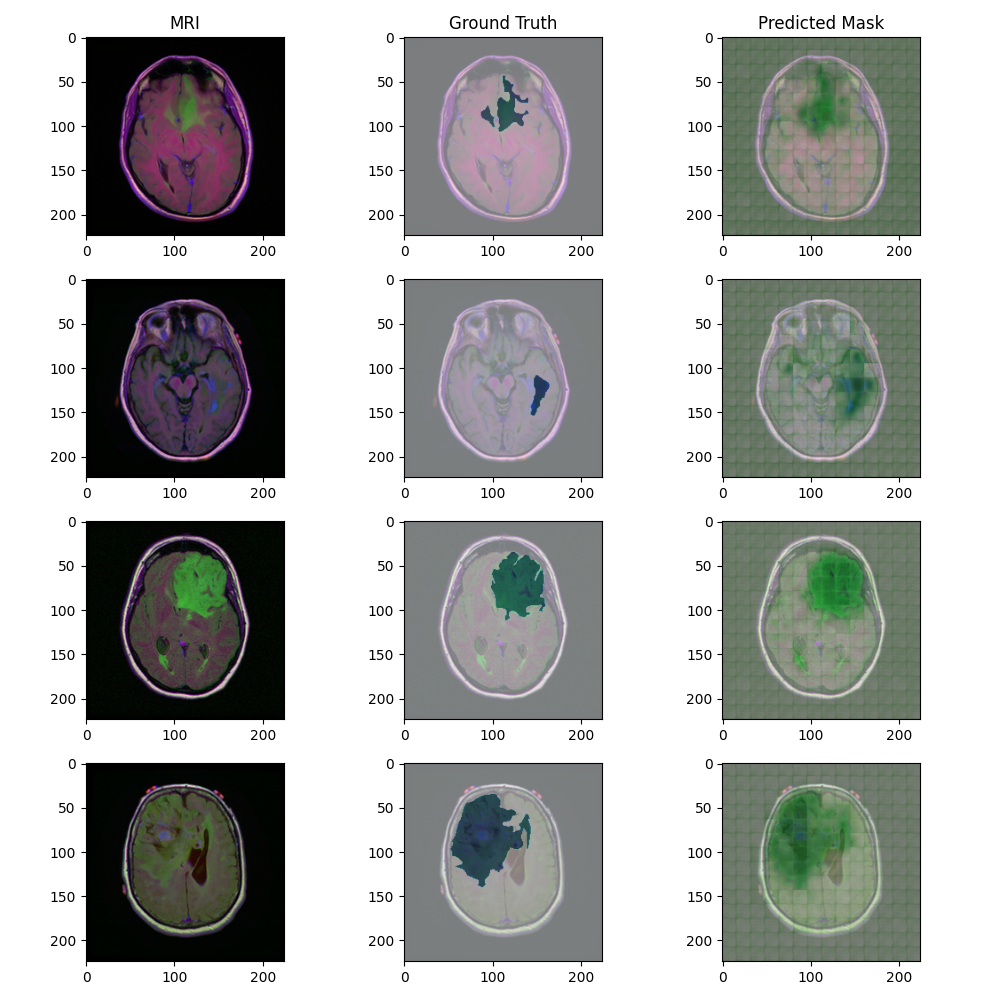
\includegraphics[width= 0.9\linewidth]{TransUnet.png}
    \caption{TransUnet result}
\end{figure}
\vspace{0.6cm}
\textbf{Summary of both Model}
\begin{itemize}
    \item Visual comparisons show that both models produce accurate segmentation masks for many cases
    \item TransUNet's predictions generally show better alignment and detail compared to UNet, indicating its robustness in handling complex segmentation tasks
    \item TransUNet proves to be a more reliable and accurate model for medical image segmentation, providing superior performance across both quantitative metrics and qualitative visualizations

\end{itemize}
\pagebreak

\subsection{Conclusion and Future Aspects}
\subsubsection{Conclusion}
In this project, I have successfully developed and evaluated two deep learning models, TransUNet and UNet, for the task of medical image segmentation. My primary goal was to accurately segment MRI images to identify regions of interest, such as tumors, which is critical for diagnosis and treatment planning
\vspace{0.3cm}
\linebreak
Overall, the TransUNet model outperformed the UNet model, demonstrating its potential as a powerful tool for medical image segmentation. The results emphasize the importance of integrating transformer-based architectures to enhance segmentation accuracy and robustness.
\vspace{0.6cm}
\subsubsection{Future Aspects}
\begin{itemize}
    \item Explore synthetic data generation methods to further augment the dataset and address class imbalances
    \item Experiment with different transformer architectures and pre-trained models to evaluate their impact on segmentation quality
    \item Incorporate additional imaging modalities (e.g., CT scans, PET scans) to create a multi-modal segmentation framework
    \item Optimize the model for real-time segmentation applications, ensuring fast and efficient processing of high-resolution medical images
    \item Develop methods to enhance the interpretability of the model’s predictions, providing insights into the decision-making process
    \item Implement explainable AI techniques to ensure the model’s outputs are transparent and trustworthy for clinical use.
\end{itemize}
\vspace{0.4cm}
Visual results indicated that while both models produced accurate segmentations, TransUNet exhibited better alignment and detail, especially in complex regions
\vspace{0.3cm}
\linebreak
These future directions aim to improve model accuracy, robustness, and clinical applicability, ultimately enhancing patient care


\pagebreak
\begin{thebibliography}{9}
    \vspace{0.9cm}

    \bibitem{KaggleDataset}
        Kaggle. \textit{Dataset of MRI images and masks}. Available at: \url{https://www.kaggle.com/}.
    
    \bibitem{UNetPaper}
        Ronneberger, O., Fischer, P., \& Brox, T. (2015). U-Net: Convolutional Networks for Biomedical Image Segmentation. \textit{arXiv preprint arXiv:1505.04597}. Available at: \url{https://arxiv.org/abs/1505.04597}.
    
    \bibitem{Model Implementation for U-net}
    Github. \textit{Implementation of U-Net model }. Available at: \url{https://github.com/uygarkurt/UNet-PyTorch/blob/main/unet.py}.
    
    \bibitem{Model Implementation for TransUNet}
    Github. \textit{Implementation of TransUNet model }. Available at: \url{https://github.com/mkara44/transunet_pytorch}.
    
    \end{thebibliography}
    

\end{document}
